\chapter{基于语谱图的端到端的语音情感识别}
\label{cha:end2end}

\section{本章引论}
\label{sec:end2end_intro}

上一章我们提出的基于情感对的语音情感识别框架取得了不错的效果,但是声学特征仍然采用传统的人工定义的特征,而这些特征无法保证一定能够反映语音中说话人的情感信息。如何从原始语音信号中学习更为有效的特征表示仍然是一个值得关注的问题。此外,当前的情感识别都是对一个完整的句子来判断的,但声学特征通常都是对语音帧抽取的,尽管可以通过对句子中所有语音帧的声学特征计算统计函数来得到整个句子的特征表示,但这样会丢失不同语音帧之间的时序信息。如何在模型中考虑特征间的时序信息同样是一个重要的问题。

近年来,深度学习的技术和工具已经飞速地发展,并且在语音信号处理领域也得到了广泛的应用。在许多的工作中,研究者逐渐开始不使用人工定义的声学特征,转而采用深度神经网络来直接从原始的语音信号上抽取相关的特征表示。这是因为深度神经网络可以从原始信号学习出更加适合任务目标的中间表示,进而使得效果提升,这被称为端到端的系统~\cite{Trigeorgis2016Adieu, Satt2017Efficient}。基于这个原因,本章将构建基于深度神经网络的端到端语音情感识别系统。

本章剩余的部分是这样安排的:首先我们将介绍CNN的结构,以及如何采用CNN从语谱图上抽取情感相关的特征表示,然后介绍RNN的结构,以及如何通过RNN对时间序列进行建模,接下来我们将通过实验对比采用人工定义特征的方法和采用CNN从语谱图抽取的特征的方法在识别效果上的差异,最后总结本章的内容。

\section{基于语谱图的端到端情感识别框架}
\label{sec:cnn_spectrogram_feature}

为了方便神经网络处理,首先会将语音句子切分成更短的等长语音段,并抽取这些语音段的语谱图(Spectrogram),然后通过卷积神经网络(Convolution Neutral Network, CNN)来从语谱图中抽取和情感相关的声学特征,接下来采用循环神经网络(Recurrent Neural Network, RNN)来建模时间序列信息,最终通过全连接神经网络建立输出RNN最后一个时间步的输出和情感类别后验概率之间的映射关系,整个系统的流程如图\ref{fig:end2end_flow}。在预测阶段,会首先计算句子包含的所有等长语音段输入模型后得到的每种情感类别的后验概率,然后对每种情感的后验概率在所有等长语音段上的平均值,平均值最大的情感类别作为模型最终识别出的句子的情感类别。

\begin{figure}[htb] % use float package if you want it here
    \vspace{-0.8cm}  %调整图片与上文的垂直距离
    \setlength{\belowcaptionskip}{0cm}   %调整图片标题与下文距离
    \centering
    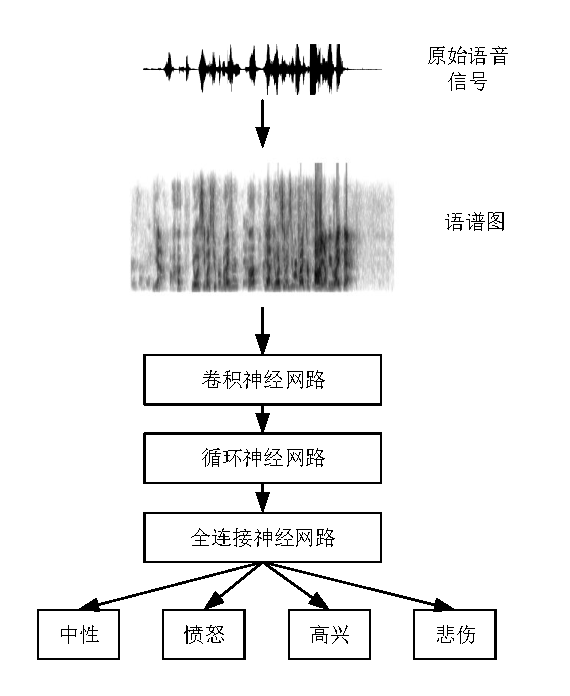
\includegraphics[height=12cm]{myfigures/end2end_flow}
    \caption{基于语谱图的端到端语音情感识别系统流程图}
    \label{fig:end2end_flow}
\end{figure}

\section{基于语谱图的卷积神经网络特征抽取}
\label{sec:cnn_spectrogram_feature}

\subsection{语谱图的定义}
\label{ssec:spectrogram}

语谱图是语音信号的不同频率的能量在时间上的变化,为了方便观测,通常会以图像的方式展示出来。图\ref{fig:spectrogram_example}给出了一张语谱图,其中横轴代表时间,纵轴代表频率,像素点的灰度值代表能量强度,颜色越深代表能量越高。假设原始语音信号为向量$\mathbf{x}$,滑动窗口的长度为$w$,语谱图可以通过下面的公式\ref{equ:spectrogram}计算出来:
\begin{equation}
\label{equ:spectrogram}
    Spectrogram(x, w) = |STFT(x, w)|^2
\end{equation}
其中$STFT(x, w)$代表对滑动窗口内的信号序列进行短时傅里叶变换(Short-Time Fourier Transform, STFT),前后两个窗口之间可以有重叠,每一个窗口经过傅里叶变换后得到的向量即为语谱图中每一个时间点对应的向量。当抽样频率大于语音信号频率的两倍时,根据奈奎斯特定理经过傅里叶变换的信号是能够恢复原始信号的,所以语谱图相对于原始语音信号没有任何信息损失,并且更容易进行频谱上的预处理,例如滤波、去噪等。通常,情感信息主要集中在语音信号的低频区域,所以我们可以采用低通滤波器对语谱图进行预处理,排除高频信息对情感识别的干扰,而原始语音信号做这样的预处理会更麻烦。

\begin{figure}[htb] % use float package if you want it here
    \vspace{-0.8cm}  %调整图片与上文的垂直距离
    \setlength{\abovecaptionskip}{-0.5cm}
    \setlength{\belowcaptionskip}{0cm}   %调整图片标题与下文距离
    \centering
    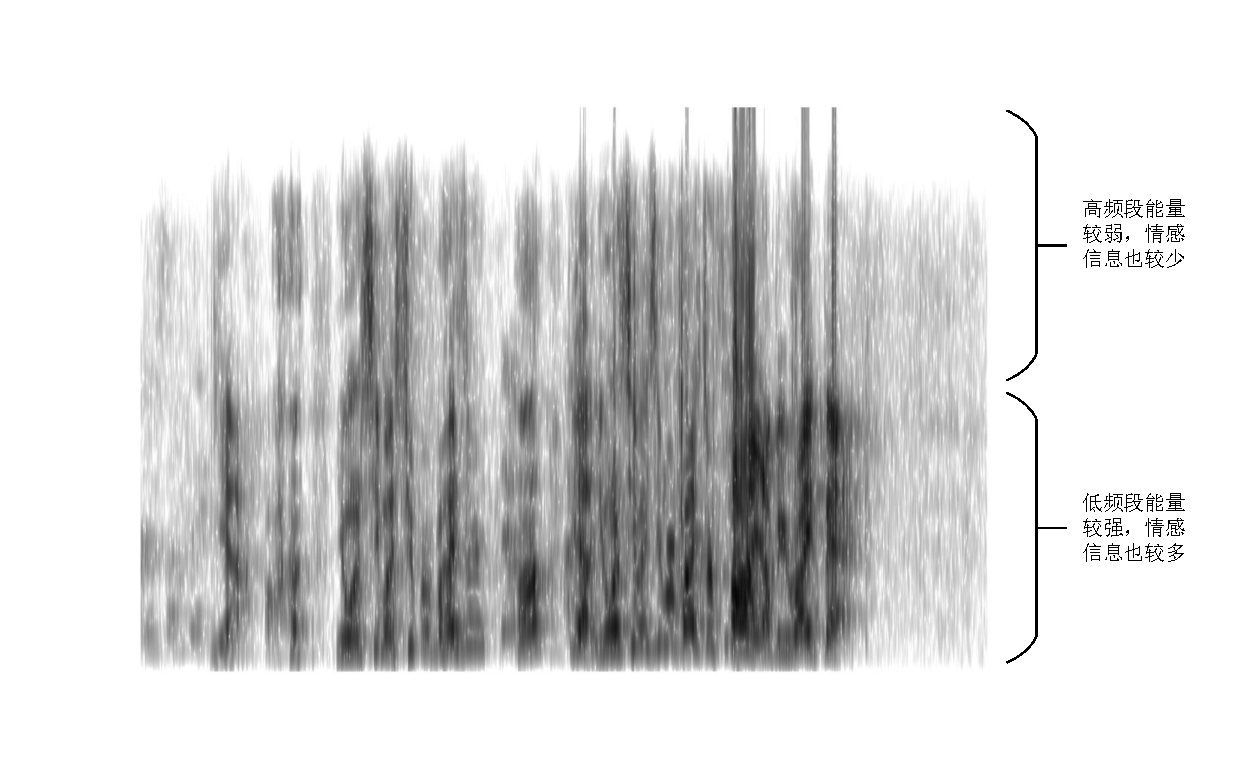
\includegraphics[height=10cm]{myfigures/spectrogram_example}
    \caption{语谱图示例}
    \label{fig:spectrogram_example}
\end{figure}

语谱图在语音信号处理领域的运用十分广泛,通常被用来观测语音信号在频谱上的变化。在语谱图上,我们可以观测到共振峰,信号强度等信息,相比于原始的语音信号,语谱图可以更直观的观测语音在时域和频域上的变化。在本章所构建的端到端的语音情感识别识别系统中,语谱图将作为模型的输入。

\subsection{卷积神经网路}
\label{ssec:cnn}

卷积神经网络(Convolution Neutral Network, CNN)是近年来被广泛使用的一种深度神经网络结构,它实际上可以被认为是将一种神经网络结构进行多份复制,然后将这些复制作用在输入的不同部分。这种网络结构可以处理规模很大的输入,同时又可以保证模型参数的数量保持不变,这使得存储模型所需的空间大大减少。这种重复利用的思想和程序设计中函数的用法很相似,就是编写一个函数的代码,然后在不同的地方调用。

为了方便表述,我们先来看一维的语音信号输入,假设我们的目的是将语音信号进行分类,输入被表示为向量$\mathbf{x}=\{x_0,x_1,...x_8\}$,CNN的单一结构,也被称为卷积核,被表示为$A$,每一个卷积核仅仅作用在一部分输入上,最后的分类输出通过一个全连接层$F$来完成,整个结构如图\ref{fig:cnn_1_layer}所示。

\begin{figure}[htb] % use float package if you want it here
    \vspace{-0.5cm}  %调整图片与上文的垂直距离
    \setlength{\belowcaptionskip}{0cm}   %调整图片标题与下文距离
    \centering
    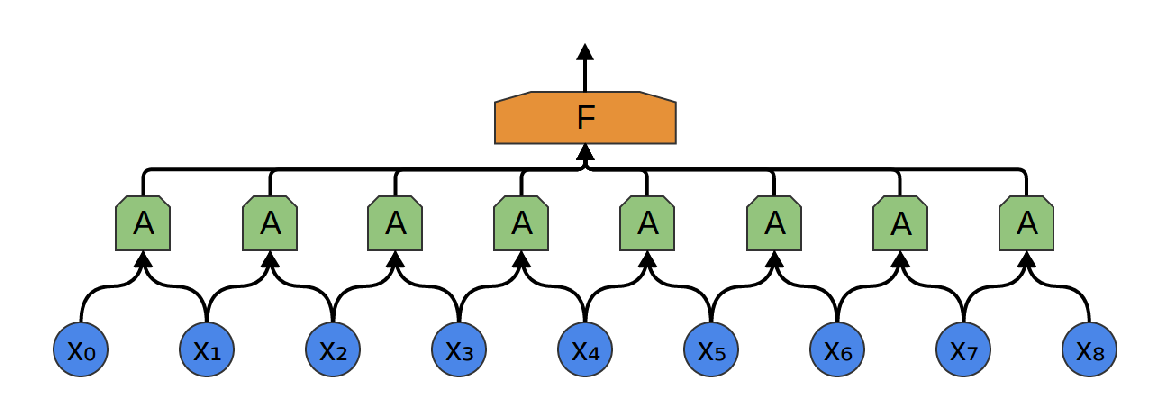
\includegraphics[height=5cm, width=12cm]{myfigures/cnn_1_layer}
    \caption{一维卷积神经网络(单卷积层)}
    \label{fig:cnn_1_layer}
\end{figure}

通常一个CNN网络会有多个卷积核,每一个卷积核代表对一小段输入的特征表示。此外,CNN可以堆叠多层,假设我们有一组新的卷积核$B$,则可以在$A$上面再叠加一层$B$,以此来得到更高级,更抽象的特征,结构如图\ref{fig:cnn_2_layer}所示。

\begin{figure}[htb] % use float package if you want it here
    \vspace{-0.5cm}  %调整图片与上文的垂直距离
    \setlength{\belowcaptionskip}{0cm}   %调整图片标题与下文距离
    \centering
    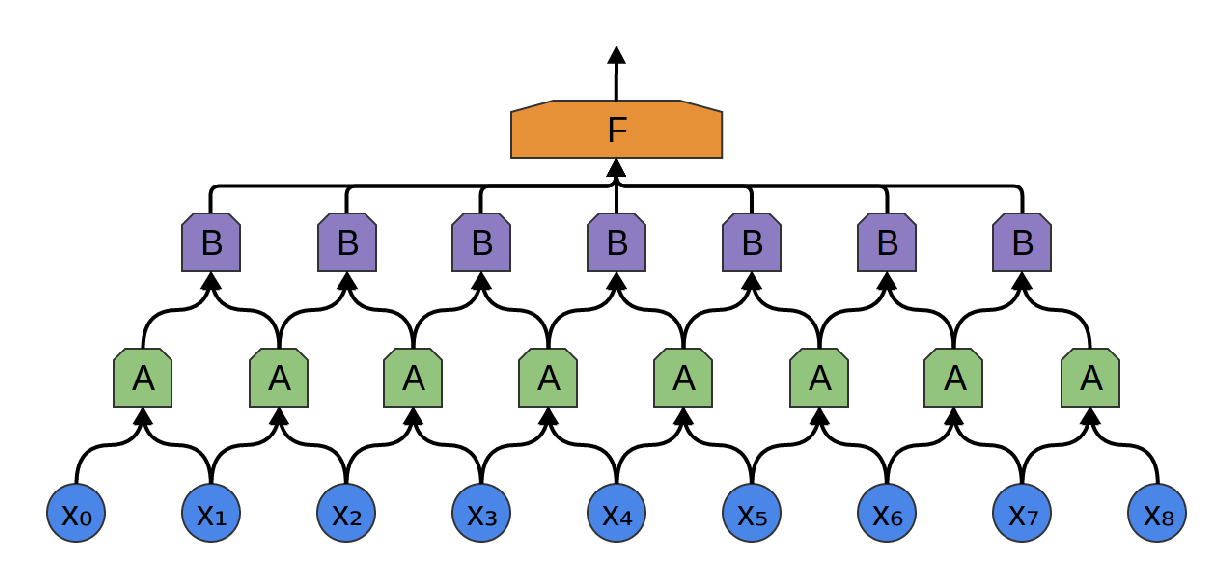
\includegraphics[height=6cm, width=12cm]{myfigures/cnn_2_layer}
    \caption{一维卷积神经网络(双卷积层)}
    \label{fig:cnn_2_layer}
\end{figure}

CNN通常还会在后面加一层池化层(Pooling Layer),目的是通过计算输入特征的统计量来保证不变性,这种不变性包括平移、旋转、尺度的不变性等。此外,还可以对输入进行降维,并且使得网络能够作用在更大的输入段上。最大值池化层(Max-Pooling Layer)是一种被广泛使用的池化层,它的目的是从上一层的每一块输出中的找出最大值,因为通常最大值最能够反映一块输出的特性,图\ref{fig:cnn_layer_pooling}给出了最大值池化层的使用方式。

\begin{figure}[htb] % use float package if you want it here
    \vspace{-0.5cm}  %调整图片与上文的垂直距离
    \setlength{\belowcaptionskip}{0cm}   %调整图片标题与下文距离
    \centering
    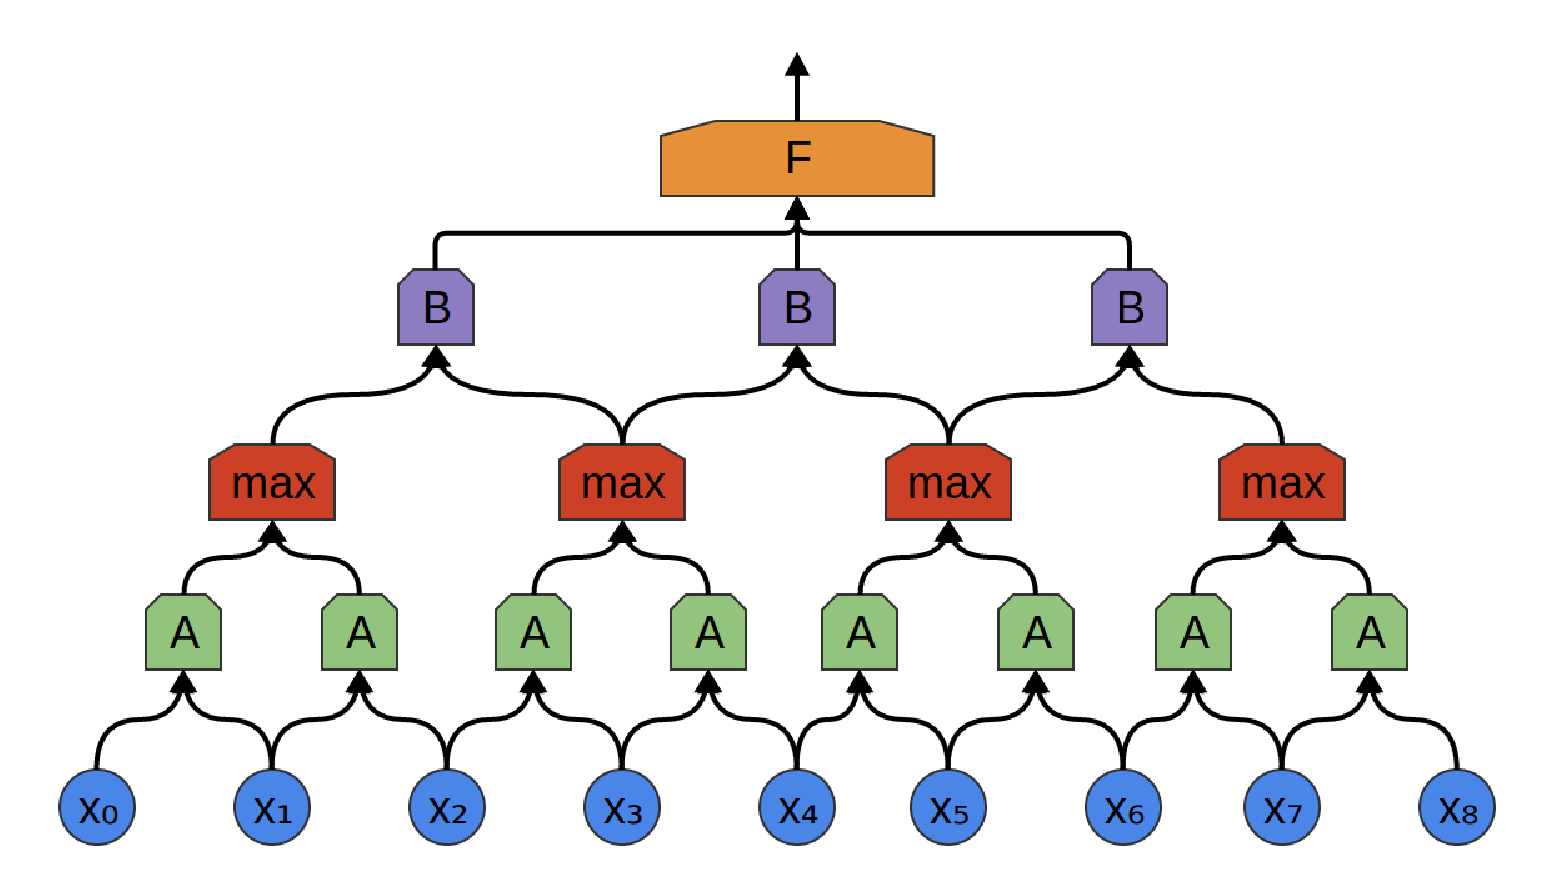
\includegraphics[height=7cm, width=12cm]{myfigures/cnn_layer_pooling}
    \caption{一维卷积神经网络(卷积层+池化层+卷积层)}
    \label{fig:cnn_layer_pooling}
\end{figure}

前面的例子主要介绍的是CNN如何处理一维的输入向量,但语谱图属于二维的输入矩阵,所以我们需要将网络结构扩展到可以处理二维输入矩阵。假设我们有输入矩阵$\mathbf{X}=\{x_{i,j}, i=0,1,...,8; j=0,1,...,8\}$,则CNN的处理将会变成图\ref{fig:cnn_layer_pooling_2dim}的方式。此时,卷积层的卷积核作用在一个二维小块上,然后得到这个小块的特征表示。

\begin{figure}[htb] % use float package if you want it here
    \vspace{-0.5cm}  %调整图片与上文的垂直距离
    \setlength{\belowcaptionskip}{0cm}   %调整图片标题与下文距离
    \centering
    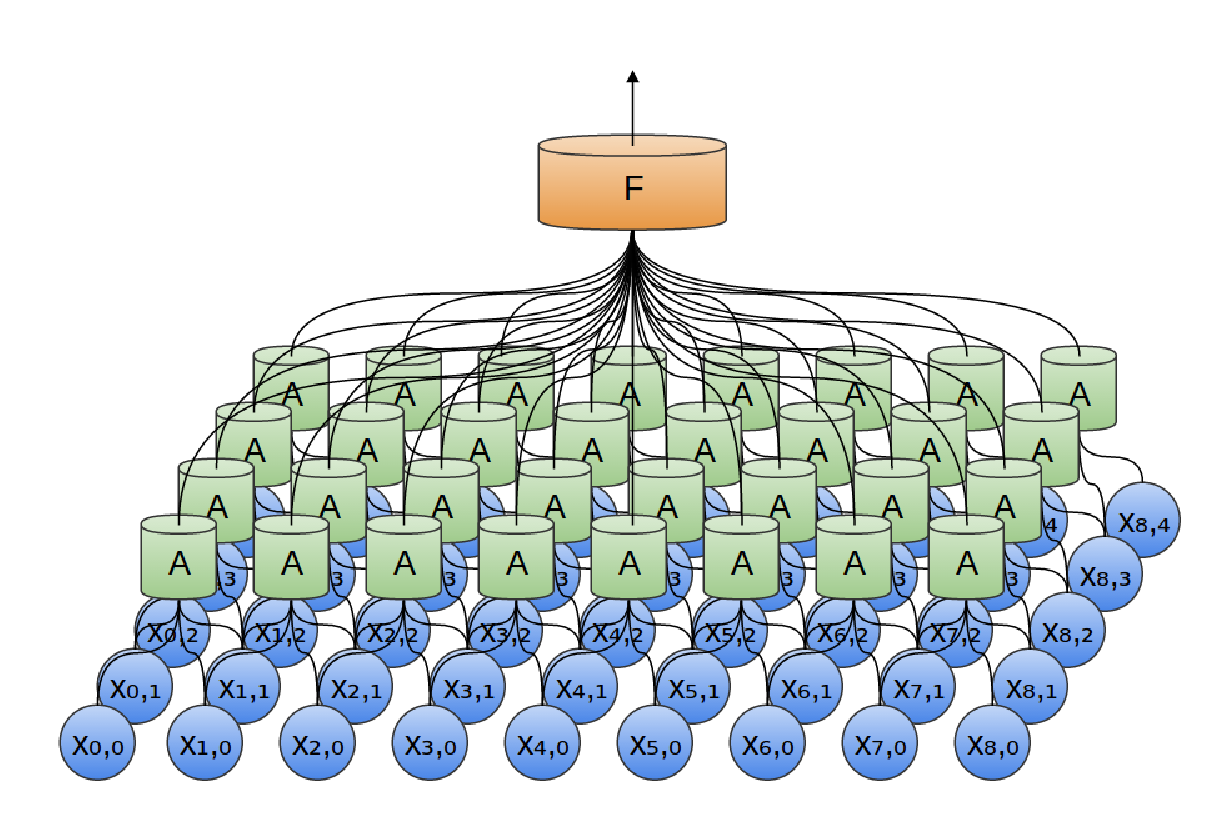
\includegraphics[height=8cm, width=12cm]{myfigures/cnn_layer_pooling_2dim}
    \caption{二维卷积神经网络(卷积层)}
    \label{fig:cnn_layer_pooling_2dim}
\end{figure}

\subsection{基于语谱图的卷积神经网络特征抽取}
\label{ssec:cnn_spectrogram_feature_extract}

CNN最早用在计算机视觉领域,因为它的处理机制和人眼感知图像的机制很类似。语谱图也可以被看做是一张图像,将CNN作为整个深度神经网络中最开始的结构可以起到特征提取的作用。相比于传统的人工定义的声学特征,CNN的训练是取决于最后的分类目标的,所以可以通过CNN得到更加符合当前任务的特征表示。此外,由于CNN是整个深度神经网络模型的一部分,所以当模型中还存在RNN时,抽取特征时还将会考虑到时序信息。通过CNN将语谱图转化为和情感相关的中间表示,就可以为后面的情感分类提供和情感相关的特征输入,从而替代传统语音情感识别框架中的声学特征。

\section{基于循环神经网络的时间序列建模}
\label{sec:rnn_seq_model}

\subsection{循环神经网络}
\label{ssec:rnn}

传统的全连接神经网络中,所有的输入都是相互独立的,但是一些任务需要建立序列输入的前后元素之间的关系,例如在语言模型中,需要根据前面出现的词对后面的词进行预测。循环神经网络(Recurrent Neural Network, RNN)的目的是对序列信息进行建模,它对于序列中的每一个元素都进行相同的计算,当前的输出不仅跟当前的输入相关,而且和之前的输入也相关。

图\ref{fig:rnn}是一个RNN的示意图。图中$\mathbf{x}=\{x_t, t=0,1,...,N\}$为输入序列,$\mathbf{s}=\{s_t, t=0,1,...,N\}$为隐状态序列,$\mathbf{o}=\{o_t, t=0,1,...,N\}$为输出序列,$(U, W, V)$是RNN的权重矩阵。序列中元素之间的映射关系可以通过下面的公式\ref{equ:rnn_cal_state}和公式\ref{equ:rnn_cal_output}表示:
\begin{equation}
\label{equ:rnn_cal_state}
    s_t = f(Ux_t + Ws_{t-1})
\end{equation}
\begin{equation}
\label{equ:rnn_cal_output}
    o_t = softmax(Vs_t)
\end{equation}
RNN中的隐藏状态是能够建模序列中前后元素关系的关键,因为当前时刻的隐藏状态$s_t$是和上一时刻的隐藏状态$s_{t-1}$相关的,而当前时刻的输出$o_t$和当前时刻隐藏状态$s_t$相关的,所以这使得当前时刻的输出$o_t$会考虑到之前的输入信息。

\begin{figure}[htb] % use float package if you want it here
    \vspace{-0.8cm}  %调整图片与上文的垂直距离
    \setlength{\belowcaptionskip}{0cm}   %调整图片标题与下文距离
    \centering
    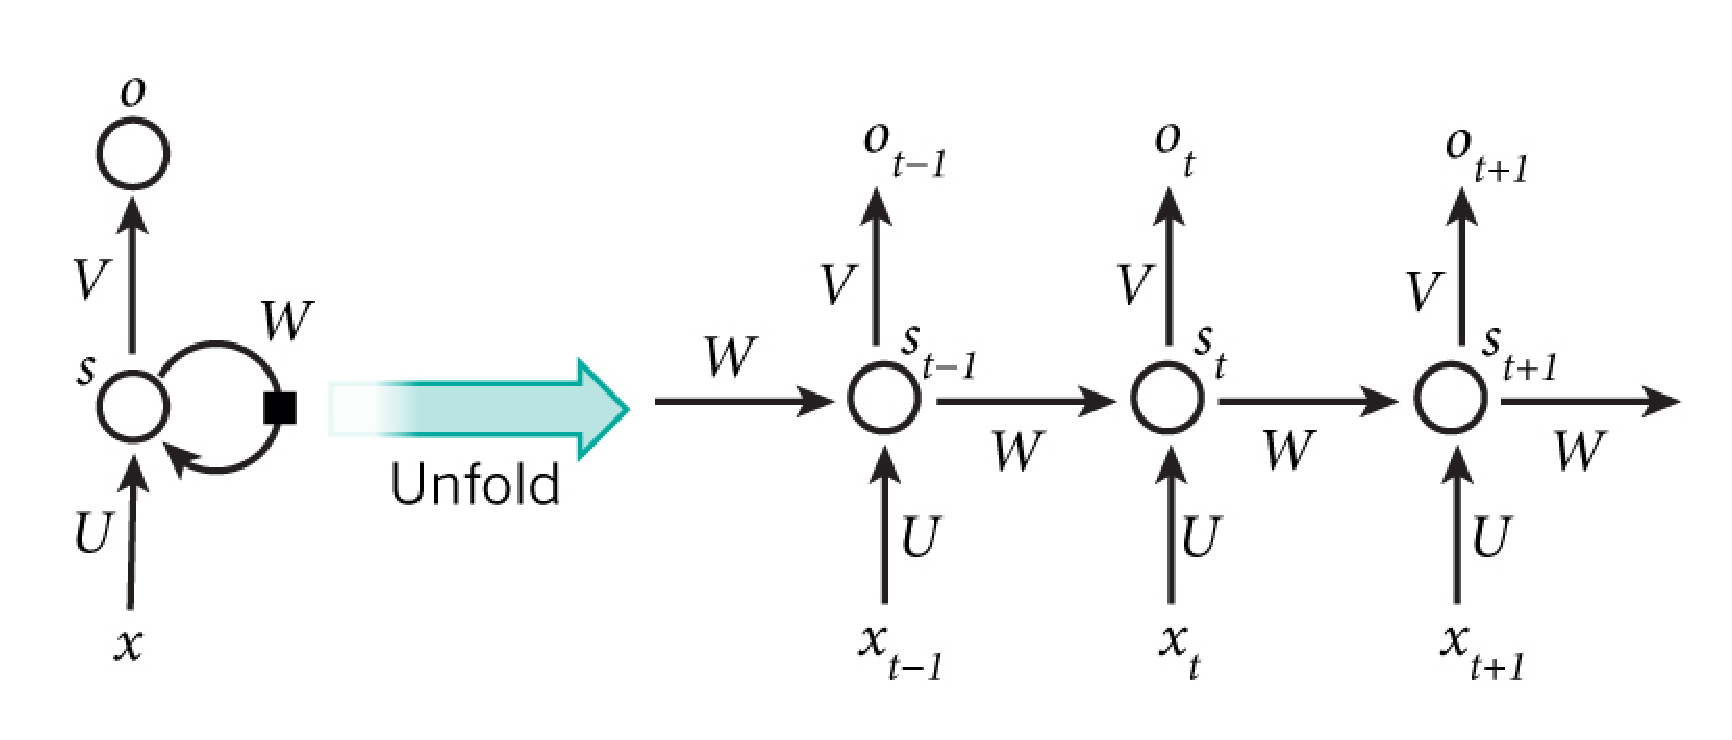
\includegraphics[height=5cm, width=12cm]{myfigures/rnn}
    \caption{循环神经网络}
    \label{fig:rnn}
\end{figure}

对于普通的RNN,当序列时间长度过长时,由于链式乘法规则,会导致出现梯度消失问题,从而使得网络并不能学习到太长时间的信息。这使得一些新的RNN网络结构被提出,例如长短时记忆(Long-Short Term Memory)网络,门循环单元(Gated Recurrent Unit)网络。它们的共同点都是引入了一种门函数(Gated Function)结构,使得网络在建模时序信息时,能够选择记住之前的哪些信息,这样的结构保证网络可以学习到更长时间的序列信息。此外,由于RNN通常只能考虑到从前到后的序列信息,但在许多任务中从后到前的序列信息也是很重要的。因此,一种双向的RNN结构也被提出,具体实现就是正常顺序的序列训练一个RNN,然后将序列逆序后再训练一个RNN,最后将两个RNN的输出拼接在一起,这种RNN结构被称为双向循环神经网络(Bi-Directional Recurrent Neural Network)。

\subsection{基于循环神经网络的时间序列建模}
\label{ssec:rnn_seq_model_detail}

之前我们通过CNN在语谱图上抽取出了相关的特征表示,这种特征表示也是一个时间序列,每一个时间点的输入向量是原始语音信号的频谱经过CNN抽象后得到的特征表示,所以我们可以通过RNN来建立不同时间步之间的时序关系。

由于语音情感识别的目标是对每一个语音段判别情感类别,所以并不需要RNN中所有时间点的输出,仅仅只需要最后一个时间点的输出。当得到RNN的输出后,关于时间序列的信息已经被编码到了当前的表示中,然后再采用全连接神经网络将输出映射到每种情感类别的后验概率,我们就搭建起了整个基于深度神经网络的端到端的语音情感识别系统。


\section{实验结果及分析}
\label{sec:end2end_experiment}

前面几节详细的介绍了基于深度神经网络的端到端的语音情感识别系统,下面我们将通过实验来对比采用人工定义的声学特征和在语谱图上直接抽取特征表示之间的效果差别。

\subsection{实验设置}
\label{ssec:end2end_experiment_setup}

\subsubsection{情感语音数据库}
\label{ssec:end2end_database}

本章所使用的数据库仍然为IEMOCAP情感语音数据库~\cite{Busso2008IEMOCAP},并且也只判别其中的四种情感:中性,愤怒,高兴和悲伤。与上一章不同的是我们将只考虑在对话中诱发的情感语音,不考虑基于特定文本表演的情感语音。因为基于特定文本表演的情感语音包含太强的语言学相关的信息,并不适合分析语音中包含的情感信息。在这章的实验中我们同样会采用交叉验证(5-Fold Cross Validation),但是将数据库按不同的主题分为5个部分,每次都将4个部分作为训练集,另一个部分中一个说话人的数据作为验证集,其他作为测试集,表格\ref{tab:end2end_emo_sample_num}是本实验中不同情感的句子数量:

\begin{table}[htb]
\centering
\begin{minipage}[t]{0.8\linewidth} % 如果想在表格中使用脚注,minipage是个不错的办法
\caption{IEMOCAP数据库中不同情感的句子数量}
\label{tab:end2end_emo_sample_num}
    % \begin{tabular}{p{6cm}<{\centering} p{6cm}<{\centering}}
    \begin{tabularx}{\linewidth}{X<{\centering} X<{\centering} X<{\centering} X<{\centering} X<{\centering}}
        \toprule[1.5pt]
        中性 & 愤怒 & 高兴 & 悲伤 & 总计 \\
        \midrule[1pt]
        1099 & 289 & 284 & 608 & 2280 \\
        \bottomrule[1.5pt]
    \end{tabularx}
\end{minipage}
\end{table}

\subsubsection{语谱图抽取}
\label{ssec:end2end_spectrogram_extract}

IEMOCAP数据库中的语音采用16kHz的采样频率,每个句子的时间长度为1s到30s不等。为了方便神经网络处理,我们首先将这些句子切分成3s长的语音段,不足3s的语音段暂时保留,然后对这些语音段计算语谱图,表格\ref{tab:end2end_spectrogram_setup}是计算语谱图时的参数设置。由于语音中的情感信息主要集中在低频的部分,所以我们只保留0-4kHz的频谱,避免高频段的信息产生干扰。此外,频谱分辨率代表语音帧通过傅里叶变化后得到的向量维度,每一个维度都代表一段频谱的能量。

\begin{table}[htb]
\centering
\begin{minipage}[t]{0.8\linewidth} % 如果想在表格中使用脚注,minipage是个不错的办法
\caption{语谱图计算的参数配置}
\label{tab:end2end_spectrogram_setup}
    % \begin{tabular}{p{6cm}<{\centering} p{6cm}<{\centering}}
    \begin{tabularx}{\linewidth}{X<{\centering} X<{\centering}}
        \toprule[1.5pt]
        参数名称 & 参数值 \\
        \midrule[1pt]
        滑动窗口类型 & 汉明窗(Hamming Window) \\
        滑动窗口长度 & 40ms \\
        滑动窗口偏移 & 10ms \\
        频谱范围 & 0-4kHz \\
        频谱分辨率 & 800 \\
        \bottomrule[1.5pt]
    \end{tabularx}
\end{minipage}
\end{table}

在得到语谱图后,我们通过取对数降低能量表示的取值范围,然后采用z-normalization对所有的样本进行正则化,其中均值和标准差基于语谱图中每一个频率刻度在所有样本中的所有时间的能量。在完成正则化后,还需要将不足3s的语谱图通过在末尾加0补齐到3s,这样就可以保证所有输入样本的长度是相同的。经过上述的处理后,神经网络模型的输入为正则化后的对数频谱分布,其时间长度大小为300(3000ms/10ms),频率尺度大小为400(4kHz/8kHz$\times$800)。经过语谱图抽取后,我们就可以得到神经网络模型的300$\times$400的二维矩阵输入。在矩阵中,时域每个点代表10ms语音的信息,频域中每个点代表10Hz的频带的信息。

\subsubsection{深度神经网络结构和参数}
\label{ssec:end2end_nn_topology}

在实验中我们采用CNN从语谱图中抽取特征表示,然后使用RNN建模语音信号的时序信息,最后通过全连接网络将RNN最后一个时间步的输出映射到情感类别的后验概率。在尝试了多种的神经网络结构和参数后,图\ref{fig:end2end_nn_topology}是我们当前最好效果的网络结构。其中,卷积层中的参数代表二维卷积核的长和宽;池化层的参数代表缩放的比例;循环神经网络层的参数代表节点的数量和双向网络。此外,由于不同情感的句子数量有所差异,所以在训练时需要对误差函数(Loss Function)乘以权重,这个权重和样本对应的情感类别在数据库中的句子数量成反比,这样可以保证模型不会对样本数量多的情感产生偏好。还有就是我们最后需要得到整个句子的情感类别,所以将会对当前句子切分得到的所有语音段计算不同情感的后验概率,然后将所有语音段的输出结果取平均值,最后将平均值最大的那种情感作为当前句子的情感识别结果。

\begin{figure}[htb] % use float package if you want it here
    \vspace{-0.8cm}  %调整图片与上文的垂直距离
    \setlength{\belowcaptionskip}{0cm}   %调整图片标题与下文距离
    \centering
    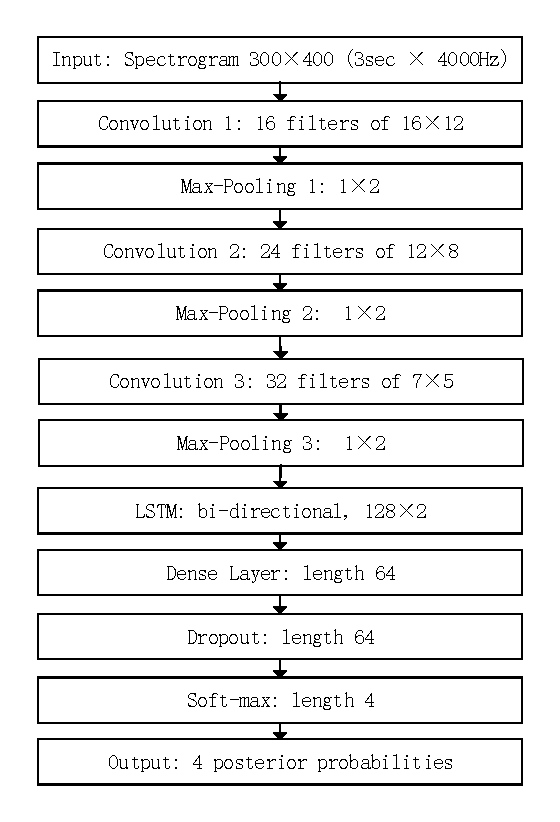
\includegraphics[height=14cm]{myfigures/end2end_nn_topology}
    \caption{深度神经网络结构}
    \label{fig:end2end_nn_topology}
\end{figure}

\subsection{实验结果}
\label{ssec:end2end_experiment_result}

实验结果主要可以分为两个部分,第一部分主要比较了基于人工定义特征的方法和基于语谱图抽取特征的方法之间识别率的差异;第二部分主要通过图像来展示语谱图通过CNN后得到的特征表示,从而进一步证明这种抽取特征的方式能够关注到语谱图中的一些特定模式信息。

\subsubsection{准确率对比}
\label{sssec:end2end_acc_comp}

本次实验的评价指标仍然是加权准确率(Weighted Accuracy, WA)和不加权准确率(Unweighted Accuracy, UA),在下面的表\ref{tab:acc_end2end}中,我们展示了以前采用传统声学特征的工作在IEMOCAP数据集上取得的最好的结果~\cite{Lee2015High}、同样的特征集在我们设计的神经网络模型上的结果、以及语谱图作为输入在我们神经网络模型上的结果。其中,“最佳结果”代表之前在传统声学特征集上取得的最好的结果~\cite{Lee2015High},“神经网络”代表在本章设计的神经网络模型下的结果。将传统特征作为我们设计的神经网络的输入时,每一个时间点的输入会从频谱能量变为传统的声学特征向量。此外,将原始语音信号的作为我们设计的神经网络的输入时,将只对时域进行卷积,因为语音信号是一维的。从实验结果中我们可以看出,当通过深度神经网络直接在语谱图上抽取特征表示时,相比于采用传统声学特征的方法,不仅在WA上取得了明显的提升,而且在UA上也取得了相近的结果。这证明采用神经网络在语谱图上抽取的特征表示相比于传统声学特征更能够反映语音中的情感信息。此外,采用语谱图也可以取得比原始语音信号更好的结果,这是因为我们只保留0-4kHz的频段,而情感信息主要分布在低频段,所以可以过滤到高频段的干扰信息。

\begin{table}[htb]
\centering
\begin{minipage}[t]{1.0\linewidth} % 如果想在表格中使用脚注,minipage是个不错的办法
\caption{不同方法的准确率}
\label{tab:acc_end2end}
    % \begin{tabular}{p{6cm}<{\centering} p{6cm}<{\centering}}
    \begin{tabularx}{\linewidth}{X<{\centering} X<{\centering} X<{\centering}}
        \toprule[1.5pt]
        模型 & WA & UA \\
        \midrule[1pt]
        传统声学特征(最佳结果)~\cite{Lee2015High} & 63.90\% & 62.80\% \\
        传统声学特征(神经网络) & 62.41\% & 60.02\% \\
        原始语音信号(神经网络) & 64.57\% & 61.43\% \\
        语谱图(神经网络) & \textbf{67.30\%} & \textbf{62.00\%} \\
        \bottomrule[1.5pt]
    \end{tabularx}
\end{minipage}
\end{table}

\subsubsection{基于卷积神经网络的特征表示}
\label{sssec:end2end_cnn_feature}

为了进一步观察深度神经网络在语谱图上学习到了什么,我们将最后一层CNN的输出以图像的方式展示出来。下面图\ref{fig:cnn_spectrogram}和图\ref{fig:cnn_activation}展示了一段中性语音的语谱图和最后一层CNN中具有代表性的两个卷积核的输出值,其中横轴代表时间,纵轴代表频率,红色代表高能量,蓝色代表低能量。从图\ref{fig:cnn_activation}中(a)的激活输出中可以观察到这个卷积核学习到了语谱图中垂直方向的模式信息,而从(b)的激活输出中则可以观察到另一个卷积核学习到了语谱图水平方向的模式信息。其他情感的语音在这两个卷积核上也可以观察到这样的现象。这些实验数据表明CNN可以从原始语谱图中捕捉到关于关于语音时域和频域的相关信息。

\begin{figure}[htb] % use float package if you want it here
    \vspace{-0cm}  %调整图片与上文的垂直距离
    \setlength{\belowcaptionskip}{0cm}   %调整图片标题与下文距离
    \centering
    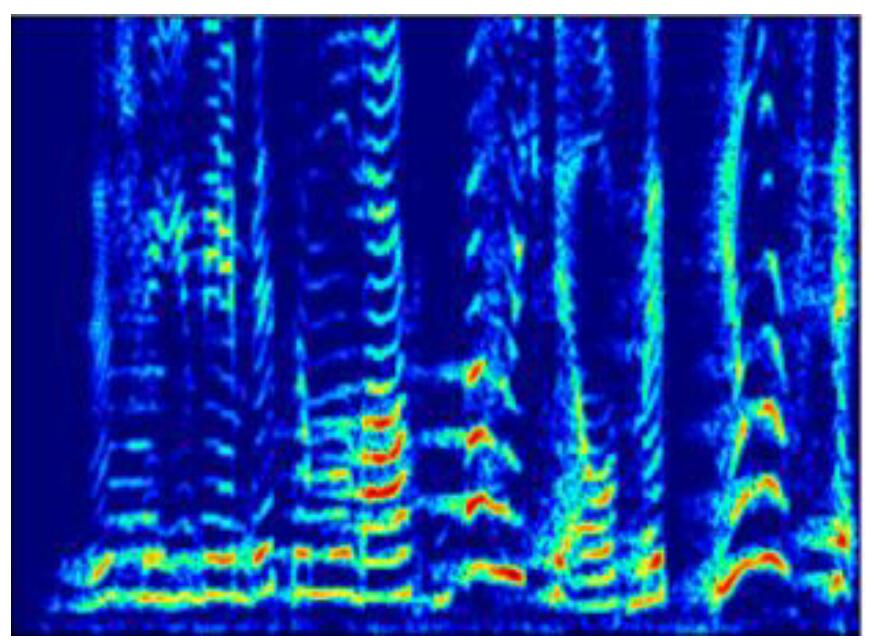
\includegraphics[height=5cm]{myfigures/cnn_spectrogram}
    \caption{原始语谱图}
    \label{fig:cnn_spectrogram}
\end{figure}

\begin{figure}[htb]
    \vspace{-0.8cm}  %调整图片与上文的垂直距离
    \setlength{\belowcaptionskip}{0cm}   %调整图片标题与下文距离
    \begin{minipage}{0.48\textwidth}
        \centering
        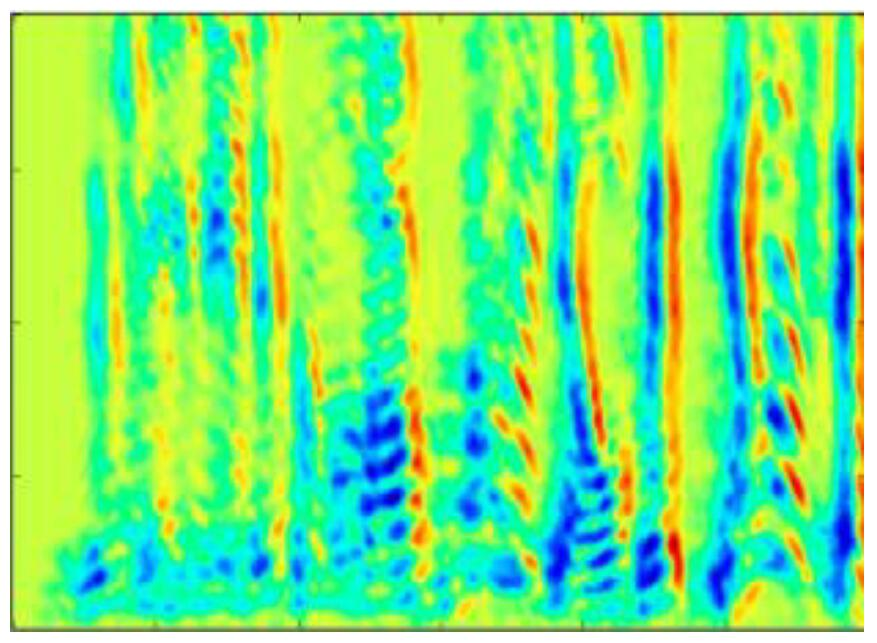
\includegraphics[height=5cm]{myfigures/cnn_vertical}
        \centerline{(a) 垂直方向模式}\medskip
    \end{minipage}\hfill
    \begin{minipage}{0.48\textwidth}
        \centering
        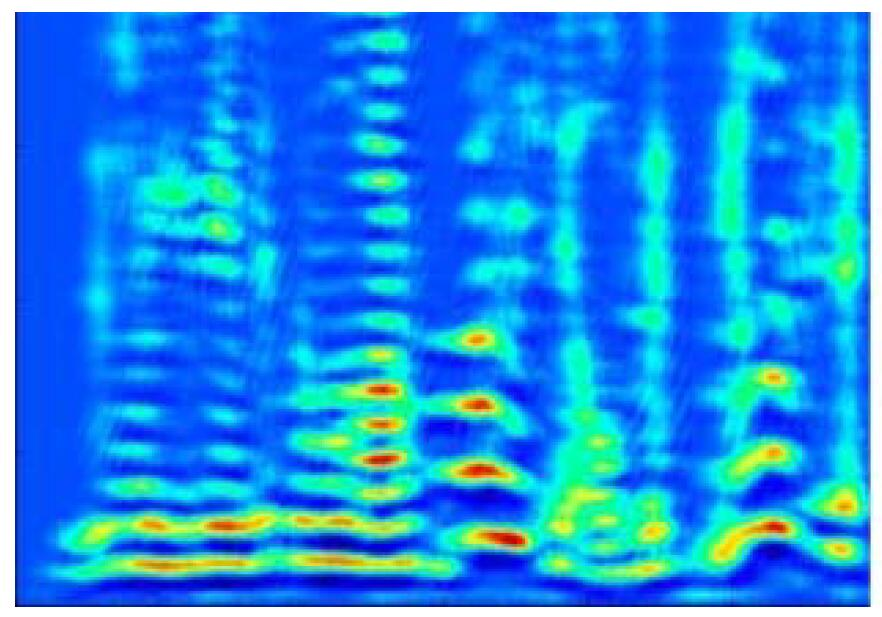
\includegraphics[height=5cm]{myfigures/cnn_horizontal}
        \centerline{(b) 水平方向模式}\medskip
    \end{minipage}
\caption{卷积神经网络中两个卷积核的激活输出}
\label{fig:cnn_activation}
\end{figure}

\section{本章小结}
\label{sec:end2end_summary}

本章我们介绍了基于深度神经网络的端到端的语音情感识别系统,首先通过CNN来直接从语谱图上抽取和情感相关的特征表示,然后采用RNN来建模语音信号的时序关系,最后通过一个全连接神经网络将RNN最后一个时间步的输出映射到不同情感的后验概率。在情感语音数据库IEMOCAP上,相比于之前基于传统声学特征的方法,基于语谱图的端到端系统可以取得更好的识别率。